\subsubsection{Tích hợp độ chệch}
\paragraph{Trường hợp $\sigma(1) \neq 1$\\}

Để hợp nhất phép tính affine về một phép nhân ma trận thuần nhất duy nhất, thành phần độ chệch có thể được tích hợp trực tiếp vào ma trận trọng số thông qua kỹ thuật tọa độ thuần nhất, tương đương với việc bổ sung một nơ-ron giả mang giá trị bất biến bằng $1$.

Theo quy ước này, véc-tơ kích hoạt tại lớp $l-1$ và ma trận trọng số tại lớp $l$ được mở rộng lần lượt thành $\hat{\mathbf{a}}^{(l-1)} \in \mathbb{R}^{n_{l-1} + 1}$ và $\hat{\mathbf{W}}^{(l)} \in \mathbb{R}^{n_l \times (n_{l-1} + 1)}$. 
Ma trận trọng số mở rộng $\hat{\mathbf{W}}^{(l)}$ thu được bằng cách ghép véc-tơ độ chệch $\mathbf{w}_0^{(l)}$ vào cột đầu tiên của ma trận trọng số $\mathbf{W}^{(l)}$:

\begin{equation}
    \hat{\mathbf{W}}^{(l)} = \begin{bmatrix}
        w_{10}^{(l)} & w_{11}^{(l)} & w_{12}^{(l)} & \dots & w_{1, n_{l-1}}^{(l)} \\
        w_{20}^{(l)} & w_{21}^{(l)} & w_{22}^{(l)} & \dots & w_{2, n_{l-1}}^{(l)} \\
        \vdots & \vdots & \vdots & \ddots & \vdots \\
        w_{n_l 0}^{(l)} & w_{n_l 1}^{(l)} & w_{n_l 2}^{(l)} & \dots & w_{n_l, n_{l-1}}^{(l)}
    \end{bmatrix} = \left[ \mathbf{w}_0^{(l)} \;\middle|\; \mathbf{W}^{(l)} \right] \in \mathbb{R}^{n_l \times (n_{l-1} + 1)},
\end{equation}

đồng thời véc-tơ kích hoạt mở rộng tương ứng được xác định bởi:

\begin{equation}
    \hat{\mathbf{a}}^{(l-1)} = \begin{bmatrix} 
        1 \\ 
        a_1^{(l-1)} \\ 
        a_2^{(l-1)} \\ 
        \vdots \\ 
        a_{n_{l-1}}^{(l-1)} 
    \end{bmatrix} = \begin{bmatrix} 1 \\ \mathbf{a}^{(l-1)} \end{bmatrix} \in \mathbb{R}^{n_{l-1} + 1}.
\end{equation}

Khi đó, phương trình lan truyền tiến tính véc-tơ tiền kích hoạt $\mathbf{z}^{(l)}$ được rút gọn thành một phép nhân ma trận thuần túy:

\begin{equation}
    \mathbf{z}^{(l)} = \hat{\mathbf{W}}^{(l)} \hat{\mathbf{a}}^{(l-1)}.
\end{equation}
\begin{equation}
\mathbf{a}^{(l)} = \sigma(\mathbf{z}^{(l)}).
\end{equation}

Quy ước trên cho phép xử lý véc-tơ độ chệch tương đương như một véc-tơ trọng số liên kết từ nơ-ron giả, đồng thời véc-tơ kích hoạt bao hàm ngầm định giá trị chệch thông qua tọa độ thuần nhất (Hình~\ref{4.8}). 

Để mở rộng toàn bộ quá trình lan truyền tiến trên một lô dữ liệu gồm $m$ mẫu huấn luyện, ma trận đặc trưng đầu vào mở rộng $\hat{\mathbf{X}} \in \mathbb{R}^{(n_0 + 1) \times m}$ được hình thành bằng cách ghép thêm một hàng gồm toàn chữ số $1$ vào phía trên ma trận dữ liệu:

\begin{equation}
    \hat{\mathbf{X}} = \hat{\mathbf{A}}^{(0)} = \begin{bmatrix}
        1 & 1 & \dots & 1 \\
        \mathbf{x}^{(1)} & \mathbf{x}^{(2)} & \dots & \mathbf{x}^{(m)}
    \end{bmatrix} = \begin{bmatrix} \mathbf{1}_m^\top \\ \mathbf{X} \end{bmatrix} \in \mathbb{R}^{(n_0 + 1) \times m},
\end{equation}
% trong đó $\mathbf{1}_m = [1, 1, \dots, 1]^\top \in \mathbb{R}^m$ là véc-tơ dùng để mô hình hóa hàng độ chệch. 

Tương tự, ma trận kích hoạt mở rộng tại mỗi lớp ẩn $l \in \{1, 2, \dots, L-1\}$ được xác định bởi:

\begin{equation}
    \hat{\mathbf{A}}^{(l)} = \begin{bmatrix}
        1 & 1 & \dots & 1 \\
        \mathbf{a}^{(l, 1)} & \mathbf{a}^{(l, 2)} & \dots & \mathbf{a}^{(l, m)}
    \end{bmatrix} = \begin{bmatrix} \mathbf{1}_m^\top \\ \mathbf{A}^{(l)} \end{bmatrix} \in \mathbb{R}^{(n_l + 1) \times m},
\end{equation}
với $\mathbf{a}^{(l, i)} \in \mathbb{R}^{n_l}$ là véc-tơ kích hoạt tại lớp $l$ của mẫu huấn luyện thứ $i$.

Khi đó, quá trình lan truyền tiến cho toàn bộ lô dữ liệu tại mỗi lớp $l \in \{1, 2, \dots, L\}$ được tính toán qua hai bước:
\begin{align}
    \mathbf{Z}^{(l)} &= \hat{\mathbf{W}}^{(l)} \hat{\mathbf{A}}^{(l-1)}, \\
    \mathbf{A}^{(l)} &= \sigma^{(l)}\left(\mathbf{Z}^{(l)}\right),
\end{align}
% trong đó:
% \begin{itemize}
%     \item $\hat{\mathbf{W}}^{(l)} \in \mathbb{R}^{n_l \times (n_{l-1} + 1)}$ là ma trận trọng số mở rộng, bao gồm cả cột trọng số chệch $\mathbf{w}_0^{(l)}$ ở vị trí đầu tiên.
%     \item $\mathbf{Z}^{(l)} \in \mathbb{R}^{n_l \times m}$ là ma trận tiền kích hoạt cho $m$ mẫu tại lớp $l$.
%     \item $\mathbf{A}^{(l)} \in \mathbb{R}^{n_l \times m}$ là ma trận kích hoạt tương ứng sau khi áp dụng hàm kích hoạt phi tuyến $\sigma^{(l)}$ theo từng phần tử.
% \end{itemize}

Tại lớp đầu ra ($l = L$), ma trận dự đoán của toàn bộ lô dữ liệu là $\mathbf{A}^{(L)} \in \mathbb{R}^{n_L \times m}$. Giá trị này được đưa trực tiếp vào hàm mất mát để đánh giá sai số và không cần mở rộng thêm hàng số $1$.

\begin{figure}[H]
    \centering
    \includegraphics[width=\linewidth]{Images/04_Images/8.png}
    \caption{Trường hợp tích hợp độ chệch với $\sigma(1) \neq 1$}
    \label{4.8}
\end{figure}

\paragraph{Trường hợp $\sigma(1) = 1$\\}

Một đặc tính thuận lợi khi sử dụng các hàm kích hoạt như ReLU ($\sigma_{\text{ReLU}}(1) = \max(1, 0) = 1$) hoặc hàm đồng nhất là khả năng tự động duy trì thành phần tọa độ thuần nhất qua từng lớp mà không cần thao tác ghép nối thủ công véc-tơ $\mathbf{1}_m$ sau mỗi bước kích hoạt.

Ma trận trọng số mở rộng tại lớp $l$ : $\overline{\mathbf{W}}^{(l)} \in \mathbb{R}^{(n_l + 1) \times (n_{l-1} + 1)}$,  dạng ma trận khối:

\begin{align}
    \overline{\mathbf{W}}^{(l)} &= \begin{bmatrix}
        1 & 0 & 0 & \dots & 0 \\
        w_{10}^{(l)} & w_{11}^{(l)} & w_{12}^{(l)} & \dots & w_{1, n_{l-1}}^{(l)} \\
        w_{20}^{(l)} & w_{21}^{(l)} & w_{22}^{(l)} & \dots & w_{2, n_{l-1}}^{(l)} \\
        \vdots & \vdots & \vdots & \ddots & \vdots \\
        w_{n_l 0}^{(l)} & w_{n_l 1}^{(l)} & w_{n_l 2}^{(l)} & \dots & w_{n_l, n_{l-1}}^{(l)}
    \end{bmatrix} \nonumber \\
    &= \begin{bmatrix}
        1 & \mathbf{0}^\top \\
        \mathbf{w}_0^{(l)} & \mathbf{W}^{(l)}
    \end{bmatrix},
\end{align}

trong đó:
\begin{itemize}
    \item $\mathbf{0}^\top = [0, 0, \dots, 0] \in \mathbb{R}^{1 \times n_{l-1}}$.
    \item $\mathbf{w}_0^{(l)} \in \mathbb{R}^{n_l}$ là véc-tơ độ chệch gắn liền với các nơ-ron tại lớp $l$.
    \item $\mathbf{W}^{(l)} \in \mathbb{R}^{n_l \times n_{l-1}}$ là ma trận trọng số kết nối giữa lớp $l-1$ và lớp $l$.
\end{itemize}

Véc-tơ kích hoạt mở rộng tương ứng $\hat{\mathbf{a}}^{(l)} \in \mathbb{R}^{n_l + 1}$:

\begin{equation}
    \hat{\mathbf{a}}^{(l)} = \begin{bmatrix} 
        1 \\ 
        a_1^{(l)} \\ 
        a_2^{(l)} \\ 
        \vdots \\ 
        a_{n_l}^{(l)} 
    \end{bmatrix} = \begin{bmatrix} 1 \\ \mathbf{a}^{(l)} \end{bmatrix}.
\end{equation}

Nhờ cấu trúc ma trận khối này, phép nhân ma trận-vector trực tiếp bảo toàn tọa độ thuần nhất:

\begin{equation}
    \hat{\mathbf{z}}^{(l)} = \overline{\mathbf{W}}^{(l)} \hat{\mathbf{a}}^{(l-1)} = \begin{bmatrix} 1 & \mathbf{0}^\top \\ \mathbf{w}_0^{(l)} & \mathbf{W}^{(l)} \end{bmatrix} \begin{bmatrix} 1 \\ \mathbf{a}^{(l-1)} \end{bmatrix} = \begin{bmatrix} 1 \\ \mathbf{W}^{(l)} \mathbf{a}^{(l-1)} + \mathbf{w}_0^{(l)} \end{bmatrix} = \begin{bmatrix} 1 \\ \mathbf{z}^{(l)} \end{bmatrix}.
\end{equation}

Khi áp dụng hàm kích hoạt $\sigma$ (với điều kiện $\sigma(1) = 1$) theo từng phần tử lên toàn bộ véc-tơ $\hat{\mathbf{z}}^{(l)}$, trạng thái kích hoạt của lớp kế tiếp tự động đạt được dạng mở rộng chuẩn tắc:

\begin{equation}
    \hat{\mathbf{a}}^{(l)} = \sigma\left(\hat{\mathbf{z}}^{(l)}\right) = \begin{bmatrix} \sigma(1) \\ \sigma\left(\mathbf{z}^{(l)}\right) \end{bmatrix} = \begin{bmatrix} 1 \\ \mathbf{a}^{(l)} \end{bmatrix}.
\end{equation}

Nhờ tính chất bảo toàn giá trị đơn vị của hàm kích hoạt ($\sigma(1) = \sigma_{\text{ReLU}}(1) = 1$), tọa độ mở rộng tại vị trí đầu tiên của véc-tơ kích hoạt luôn được duy trì bằng $1$ qua các lớp ẩn liên tiếp. Do đó, quá trình lan truyền tiến cho một mẫu đơn lẻ được mô hình hóa bằng các phép nhân ma trận thuần nhất:

\begin{align}
    \hat{\mathbf{z}}^{(l)} &= \overline{\mathbf{W}}^{(l)} \hat{\mathbf{a}}^{(l-1)}, \\
    \hat{\mathbf{a}}^{(l)} &= \sigma^{(l)}\left(\hat{\mathbf{z}}^{(l)}\right), \quad \forall l \in \{1, 2, \dots, L-1\}.
\end{align}

Tại lớp đầu ra ($l = L$), do không còn lớp kế tiếp cần duy trì tọa độ thuần nhất, ma trận trọng số chỉ cần tích hợp véc-tơ độ chệch mà không cần bổ sung hàng $[1, \mathbf{0}^\top]$. Khi đó, $\hat{\mathbf{W}}^{(L)} = \left[\mathbf{w}_0^{(L)} \;\middle|\; \mathbf{W}^{(L)}\right] \in \mathbb{R}^{n_L \times (n_{L-1} + 1)}$, và giá trị dự đoán cuối cùng được xác định bởi:
\begin{align}
    \mathbf{z}^{(L)} &= \hat{\mathbf{W}}^{(L)} \hat{\mathbf{a}}^{(L-1)}, \\
    \mathbf{a}^{(L)} &= \sigma^{(L)}\left(\mathbf{z}^{(L)}\right) \in \mathbb{R}^{n_L}.
\end{align}

Mở rộng cho một lô dữ liệu gồm $m$ mẫu quan sát, ma trận kích hoạt mở rộng tại mỗi lớp $l \in \{0, 1, \dots, L-1\}$ có dạng:

\begin{equation}
    \hat{\mathbf{A}}^{(l)} = \begin{bmatrix}
        1 & 1 & \dots & 1 \\
        \mathbf{a}^{(l, 1)} & \mathbf{a}^{(l, 2)} & \dots & \mathbf{a}^{(l, m)}
    \end{bmatrix} = \begin{bmatrix} \mathbf{1}_m^\top \\ \mathbf{A}^{(l)} \end{bmatrix} \in \mathbb{R}^{(n_l + 1) \times m}.
\end{equation}

Hệ phương trình lan truyền tiến dạng ma trận khối cho toàn bộ lô được tổng quát hóa thành:

\begin{align}
    \hat{\mathbf{Z}}^{(l)} &= \overline{\mathbf{W}}^{(l)} \hat{\mathbf{A}}^{(l-1)}, \quad &&\hat{\mathbf{A}}^{(l)} = \sigma^{(l)}\left(\hat{\mathbf{Z}}^{(l)}\right), \quad &&\forall l \in \{1, 2, \dots, L-1\}, \\
    \mathbf{Z}^{(L)} &= \hat{\mathbf{W}}^{(L)} \hat{\mathbf{A}}^{(L-1)}, \quad &&\mathbf{A}^{(L)} = \sigma^{(L)}\left(\mathbf{Z}^{(L)}\right) \in \mathbb{R}^{n_L \times m}.
\end{align}

Xét kiến trúc mạng cụ thể trong Hình~\ref{4.9} với cấu hình số nơ-ron $\{n_0=4, n_1=3, n_2=3, n_3=3, n_4=1\}$. Với đầu vào mở rộng $\hat{\mathbf{a}}^{(0)} = [1, (\mathbf{a}^{(0)})^\top]^\top \in \mathbb{R}^5$, quá trình tính toán được thực hiện tuần tự:
\begin{align}
    \hat{\mathbf{a}}^{(l)} &= \sigma^{(l)}\left(\overline{\mathbf{W}}^{(l)} \hat{\mathbf{a}}^{(l-1)}\right) \in \mathbb{R}^4, \quad \forall l \in \{1, 2, 3\}, \\
    \mathbf{a}^{(4)} &= \sigma^{(4)}\left(\hat{\mathbf{W}}^{(4)} \hat{\mathbf{a}}^{(3)}\right) \in \mathbb{R}^1.
\end{align}
Ta có thể tóm tắt toàn bộ mạng nơ-ron bằng phương trình sau:
\begin{equation}
    \mathcal{N}\left(\mathbf{a}^{(0)}\right) = \sigma^{(4)} \Biggl( 
        \underbrace{\hat{\mathbf{W}}^{(4)} \sigma^{(3)} \biggl( 
            \underbrace{\overline{\mathbf{W}}^{(3)} \sigma^{(2)} \Bigl( 
                \underbrace{\overline{\mathbf{W}}^{(2)} \sigma^{(1)} \bigl( 
                    \underbrace{\overline{\mathbf{W}}^{(1)} \hat{\mathbf{a}}^{(0)}}_{\hat{\mathbf{z}}^{(1)}} 
                \bigr)}_{\hat{\mathbf{z}}^{(2)}} 
            \Bigr)}_{\hat{\mathbf{z}}^{(3)}} 
        \biggr)}_{\mathbf{z}^{(4)}} 
    \Biggr) = \mathbf{a}^{(4)}
\end{equation}

\begin{figure}[H]
    \centering
    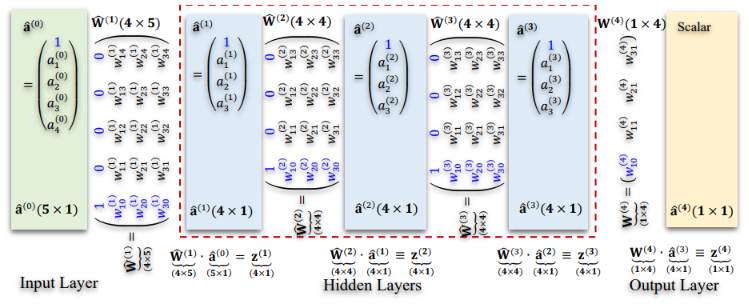
\includegraphics[width=\linewidth]{Images/04_Images/9.png}
    \caption{Trường hợp tích hợp độ chệch với $\sigma(1) = 1$}
    \label{4.9}
\end{figure}
